% Provenance (never printed): cycle 4 SVT/physique, "La planete Terre,
% l'environnement": uneven heating of the Earth, movements of the
% atmosphere, the global circulation and the climate zones; see
% sources/book1/PROVENANCE.md. Book 1, grade 8, chapter 2.
% Vocabulary guard: owns convection cell (atmospheric, descriptive), sea
% breeze and land breeze, the global winds, the global circulation. The
% Coriolis effect is told as "the Earth's rotation deflects"; Hadley and
% Ferrel cells and the intertropical convergence zone are named in prose
% only (Book 3 owns them); mantle convection is Book 2's.
\chapter{الرياح والدورة العامة للغلاف الجوي}\label{ch:g8:winds-global-circulation}

طوال قرون، اعتمدت السفن الشراعية التي تغادر موانئ أوروبا وإفريقيا متجهة
إلى الأمريكيتين على ريح ثابتة من الشرق، تهب على جانبي \omterm{def:g3:continents-and-oceans:equator}{خط الاستواء}
وحملتها عبر الأطلسي. وكان البحارة في العالم كله يعرفونها، وكانت التجارة
المبكرة مع الأمريكيتين تعتمد عليها: إنها \emph{الريح التجارية}. وحتى اليوم،
تستعمل سفن الشحن \omterm{def:g8:winds-global-circulation:global-winds}{الرياح التجارية}، والتيارات البحرية التي تحركها، لتقصير
رحلاتها.
% ledger: nos:trade-winds

\begin{omfigure}
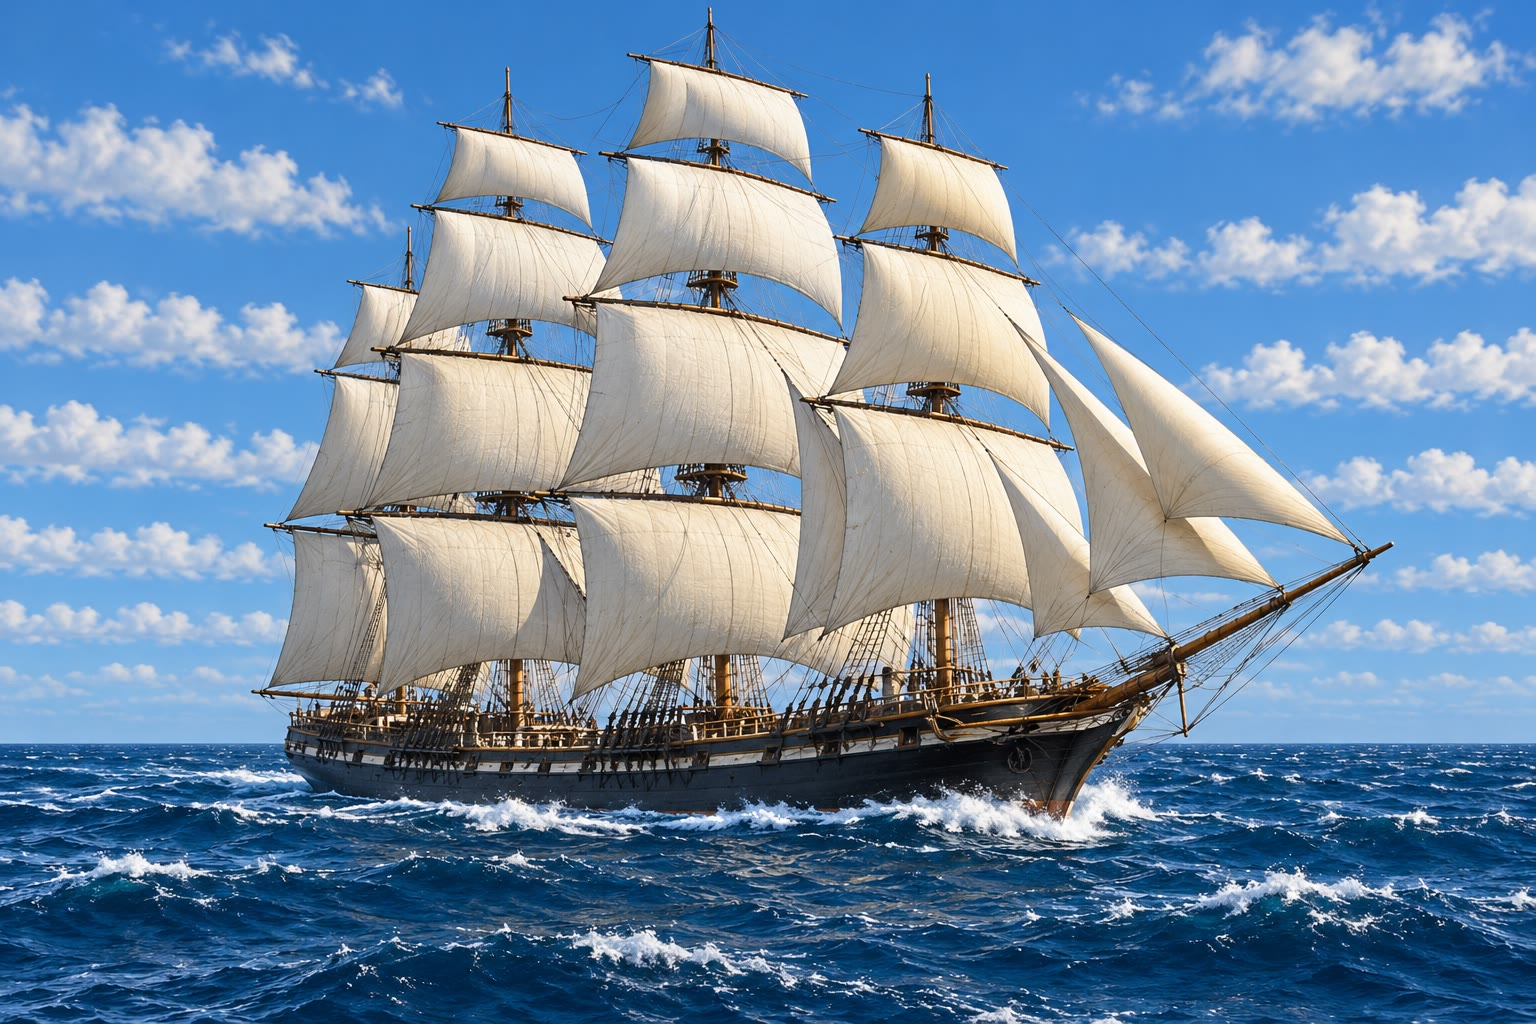
\includegraphics[width=0.62\linewidth]{images/book1/ai/g8-sailing-ship.jpg}

{\small سفينة شراعية تجري أمام ريح ثابتة في عرض \omterm{def:g2:water-on-earth:ocean}{المحيط} (رسم توضيحي مولَّد
بالذكاء الاصطناعي لمشهد عام).}
\label{fig:g8:winds-global-circulation:ship}
\end{omfigure}

لماذا تهب الريح التجارية من الشرق، ودائمًا في الأماكن نفسها؟ ولماذا توجد
\omterm{def:g5:weather-and-climate:desert}{صحارى} قرب المدارين \omterm{def:g5:weather-and-climate:rainforest}{وغابات مطيرة} قرب \omterm{def:g3:continents-and-oceans:equator}{خط الاستواء}؟ الجواب يبدأ
بالشمس.

\begin{recall}
الريح هواء متحرك (كتب الفيزياء). والهواء يضغط على كل ما يلامسه، والضغط
ينخفض مع \omterm{def:g4:world-physical-map:altitude}{الارتفاع} (\cref{ch:g8:the-atmosphere}). ويحدث \omterm{def:g1:watching-the-weather:weather}{الطقس} في
\omterm{def:g8:the-atmosphere:layers}{التروبوسفير}، الطبقة السفلى من الغلاف الجوي. وللأرض \omterm{def:g5:weather-and-climate:climate-zone}{نطاقات مناخية}: حارة
ورطبة قرب \omterm{def:g3:continents-and-oceans:equator}{خط الاستواء}، فيها \omterm{def:g5:weather-and-climate:rainforest}{غابات مطيرة}؛ \omterm{def:g5:weather-and-climate:desert}{وصحارى} حارة جافة قرب المدارين؛
ثم نطاقات معتدلة فباردة نحو \omterm{def:g3:continents-and-oceans:poles}{القطبين}
(\cref{ch:g5:weather-and-climate}).
\end{recall}

\section{الشمس تسخّن الأرض على نحو غير متساوٍ}

عند الظهر في يوم الاعتدال، تكون الشمس فوق \omterm{def:g3:continents-and-oceans:equator}{خط الاستواء} تمامًا. فتصل أشعتها
إليه شديدة الانحدار وتسقط على رقعة صغيرة من الأرض. وأبعد شمالًا أو جنوبًا،
تصل الأشعة نفسها مائلة وتنتشر على رقعة أكبر: فيتلقى كل متر مربع قدرًا أقل
من طاقتها. وعند \omterm{def:g6:latitude-longitude:latitude}{دائرة العرض} \ang{60}، تغطي الحزمة نفسها ضعف الأرض التي
تغطيها عند \omterm{def:g3:continents-and-oceans:equator}{خط الاستواء}، فيتلقى كل متر مربع نصف ما يتلقاه هناك.
% ledger: (geometry: figdata/grade-8/sunlight_spread.py, spread = 1/cos(latitude))

\begin{omfigure}
\begin{tikzpicture}[font=\footnotesize]
  \def\R{2.6}\def\w{0.2}
  \fill[blue!10] (0,0) circle (\R);
  \draw (0,0) circle (\R);
  \draw[black!50] (-\R,0) -- (\R,0);
  \draw[black!40, dashed] (0,0) -- (60:\R);
  \draw[black!40] (0,0) ++(0:0.7) arc (0:60:0.7);
  \node at (25:0.95) {\ang{60}};
  \node[anchor=east, black!60] at (-\R-0.05,0) {خط الاستواء};
  % beam at the equator: rays between y = -w and y = w
  \foreach \y in {-0.2,-0.1,0,0.1,0.2} {
    \pgfmathsetmacro{\x}{sqrt(\R*\R-\y*\y)}
    \draw[orange!80!black, -{Stealth[length=1.6mm]}] (6.2,\y) -- (\x+0.03,\y);}
  \draw[omThm, line width=2.2pt] ({sqrt(\R*\R-0.35*0.35)},-0.35) arc ({asin(-\w/\R)}:{asin(\w/\R)}:\R);
  % beam near 60 degrees: rays between y = R sin 60 - w and + w
  \pgfmathsetmacro{\yc}{\R*sin(60)}
  \foreach \d in {-0.2,-0.1,0,0.1,0.2} {
    \pgfmathsetmacro{\y}{\yc+\d}
    \pgfmathsetmacro{\x}{sqrt(\R*\R-\y*\y)}
    \draw[orange!80!black, -{Stealth[length=1.6mm]}] (6.2,\y) -- (\x+0.03,\y);}
  \draw[omThm, line width=2.2pt] ({sqrt(\R*\R-(\yc-\w)^2)},\yc-\w) arc ({asin((\yc-\w)/\R)}:{asin((\yc+\w)/\R)}:\R);
  \node[anchor=west, align=left] at (6.3,0) {الحزمة نفسها\\على رقعة صغيرة};
  \node[anchor=west, align=left] at (6.3,\yc) {الحزمة نفسها منتشرة\\على ضعف الأرض};
\end{tikzpicture}

{\small حزمتان متماثلتان من ضوء الشمس عند الظهر في يوم الاعتدال. عند \omterm{def:g3:continents-and-oceans:equator}{خط
الاستواء} تسقطان رأسيًا على رقعة صغيرة (الخط السميك)؛ وعند \omterm{def:g6:latitude-longitude:latitude}{دائرة العرض}
\ang{60} تميلان وتغطيان ضعف الأرض.}
% ledger: (geometry: figdata/grade-8/sunlight_spread.py)
\label{fig:g8:winds-global-circulation:beams}
\end{omfigure}

\begin{center}\small
\begin{tabular}{|l|c|c|c|c|c|}
\hline
\omterm{def:g6:latitude-longitude:latitude}{دائرة العرض} & \ang{0} & \ang{30} & \ang{45} & \ang{60} & \ang{75} \\
\hline
الأرض التي تغطيها الحزمة نفسها & 1 & 1.15 & 1.41 & 2 & 3.86 \\
\hline
الطاقة لكل متر مربع (\% من طاقة \omterm{def:g3:continents-and-oceans:equator}{خط الاستواء}) & 100 & 87 & 71 & 50 & 26 \\
\hline
\end{tabular}
\end{center}
% ledger: (figdata/grade-8/sunlight_spread.py main table)

بينما تدور الأرض حول الشمس، يجعل محورها المائل الشمسَ العمودية تنتقل بين
المدارين، وهذا ما يعطي الفصول (كتب الفيزياء)؛ لكن المناطق القريبة من \omterm{def:g3:continents-and-oceans:equator}{خط
الاستواء} تتلقى طوال السنة طاقة أكثر بكثير من المناطق القريبة من \omterm{def:g3:continents-and-oceans:poles}{القطبين}.
وهذا التسخين غير المتساوي هو المحرك الرئيسي للرياح: فالغلاف الجوي ينقل
الهواء الدافئ نحو \omterm{def:g3:continents-and-oceans:poles}{القطبين} والهواء البارد نحو \omterm{def:g3:continents-and-oceans:equator}{خط الاستواء}.
% ledger: mo:global-circ

\section{هواء يصعد وهواء يهبط}

الهواء الدافئ أخف من الهواء البارد: فهو يصعد، ويتدفق الهواء الأبرد \omterm{def:g2:water-on-earth:ocean}{المحيط}
به ليحل محله. وحيث يصعد الهواء، يضغط على الأرض أقل: فيكون الضغط هناك
منخفضًا. وحيث يهبط الهواء، يضغط أكثر: فيكون الضغط عاليًا. وعند الأرض، تهب
الريح من الضغط العالي نحو الضغط المنخفض. فيصعد الهواء ويبرد ويهبط ثم
يعود، دائرًا في حلقة.
% ledger: jetstream:sea-breeze, mo:three-cells

\begin{definition}[خلية الحمل]\label{def:g8:winds-global-circulation:convection-cell}
\emph{خلية الحمل}\index{خلية حمل} في الغلاف الجوي حلقة من الهواء المتحرك:
هواء يسخن من الأسفل فيصعد، وينتشر في الأعلى، ويبرد ويهبط في مكان آخر،
ثم يعود على طول الأرض إلى حيث صعد. وتحت الهواء الصاعد يكون الضغط منخفضًا؛
وتحت الهواء الهابط يكون عاليًا.
\end{definition}
% ledger: jetstream:sea-breeze, mo:three-cells

\begin{inthelab}[الهواء الدافئ يصعد]
داخل البيت، قص حلزونًا من ورقة رقيقة، كقشر تفاحة، وعلّقه من مركزه بخيط.
أمسكه عاليًا فوق مشعاع تدفئة دافئ في الشتاء (ولا تمسكه أبدًا فوق لهب أو
شمعة): فيبدأ بالدوران ببطء. فالهواء الذي يسخّنه المشعاع يصعد ويدفع
الحلزون. ثم أمسكه قرب نافذة باردة: هل يدور في الاتجاه المعاكس، أم لا يدور
أصلًا؟
\end{inthelab}

يمكن أن نحس بأصغر \omterm{def:g8:winds-global-circulation:convection-cell}{خلايا الحمل} في يوم مشمس على شاطئ \omterm{def:g2:water-on-earth:ocean}{البحر}. فاليابسة \omterm{def:g2:water-on-earth:ocean}{والبحر}
يتلقيان أشعة الشمس نفسها، لكن أشعة الشمس لا تتوغل عميقًا في الأرض، بينما
ينشر \omterm{def:g2:water-on-earth:ocean}{البحر} حرارته في طبقة سميكة من الماء. ولذلك تسخن اليابسة أكثر بكثير
في النهار، وتبرد أكثر بكثير في الليل.
% ledger: jetstream:sea-breeze

\begin{omfigure}
\begin{tikzpicture}[font=\footnotesize, >={Stealth[length=2mm]}]
  \foreach \px/\title/\dir in {0/{في النهار: نسيم البحر}/1, 8.3/{في الليل: نسيم البر}/-1} {
    \begin{scope}[xshift=\px cm]
      \fill[omSea] (0,0) rectangle (3.5,0.45);
      \fill[omLithAlluv] (3.5,0) -- (3.5,0.45) -- (7,0.75) -- (7,0) -- cycle;
      \draw (0,0.45) -- (3.5,0.45) -- (7,0.75);
      \node[anchor=south] at (3.5,3.25) {\textbf{\title}};
      \node at (1.75,0.22) {البحر};
      \node at (5.6,0.3) {اليابسة};
    \end{scope}}
  % day loop: surface sea -> land, rise over land, return aloft, sink over sea
  \draw[->, omDef, line width=1.1pt] (1.2,0.8) -- (5.2,0.95);
  \draw[->, omThm, line width=1.1pt] (5.8,1.1) -- (5.8,2.4);
  \draw[->, black!60, line width=1.1pt] (5.2,2.75) -- (1.2,2.75);
  \draw[->, omDef, line width=1.1pt] (0.6,2.4) -- (0.6,1.1);
  \node[omDef] at (3.2,1.25) {نسيم البحر};
  \node at (0.6,0.75) {\textbf{ع}};
  \node at (5.8,0.95) {\textbf{م}};
  \fill[yellow!80!orange] (6.6,2.7) circle (0.25);
  \node[anchor=north, align=center] at (1.75,-0.1) {بحر أبرد};
  \node[anchor=north, align=center] at (5.3,-0.1) {يابسة أدفأ};
  % night loop: surface land -> sea, rise over sea, return aloft, sink over land
  \begin{scope}[xshift=8.3cm]
    \draw[->, omDef, line width=1.1pt] (5.2,1.0) -- (1.2,0.8);
    \draw[->, omThm, line width=1.1pt] (0.6,1.1) -- (0.6,2.4);
    \draw[->, black!60, line width=1.1pt] (1.2,2.75) -- (5.2,2.75);
    \draw[->, omDef, line width=1.1pt] (5.8,2.4) -- (5.8,1.15);
    \node[omDef] at (3.2,1.3) {نسيم البر};
    \node at (0.6,0.75) {\textbf{م}};
    \node at (5.8,1.0) {\textbf{ع}};
    \fill[black!25] (6.6,2.7) circle (0.25); \fill[white] (6.72,2.78) circle (0.21);
    \node[anchor=north, align=center] at (1.75,-0.1) {بحر أدفأ};
    \node[anchor=north, align=center] at (5.3,-0.1) {يابسة أبرد};
  \end{scope}
\end{tikzpicture}

{\small \omterm{def:g8:winds-global-circulation:breezes}{نسيم البحر} \omterm{def:g8:winds-global-circulation:breezes}{ونسيم البر}: خليتا حمل صغيرتان تدوران في اتجاهين
متعاكسين. الأسهم الحمراء: هواء دافئ صاعد؛ ع وم: ضغط عالٍ وضغط منخفض عند
الأرض. وفي النهار تبلغ الحلقة \omterm{def:g4:world-physical-map:altitude}{ارتفاع} 1000 إلى
\qty{1500}{m}.}
% ledger: jetstream:sea-breeze
\label{fig:g8:winds-global-circulation:breezes}
\end{omfigure}

\begin{definition}[نسيم البحر ونسيم البر]\label{def:g8:winds-global-circulation:breezes}
\emph{نسيم البحر}\index{نسيم البحر} ريح تهب من \omterm{def:g2:water-on-earth:ocean}{البحر} نحو اليابسة في
النهار، حين تكون اليابسة أدفأ من \omterm{def:g2:water-on-earth:ocean}{البحر}. و\emph{نسيم البر}\index{نسيم البر}
يهب من اليابسة نحو \omterm{def:g2:water-on-earth:ocean}{البحر} في الليل، حين تصير اليابسة أبرد من
\omterm{def:g2:water-on-earth:ocean}{البحر}.
\end{definition}
% ledger: jetstream:sea-breeze

\begin{omfigure}
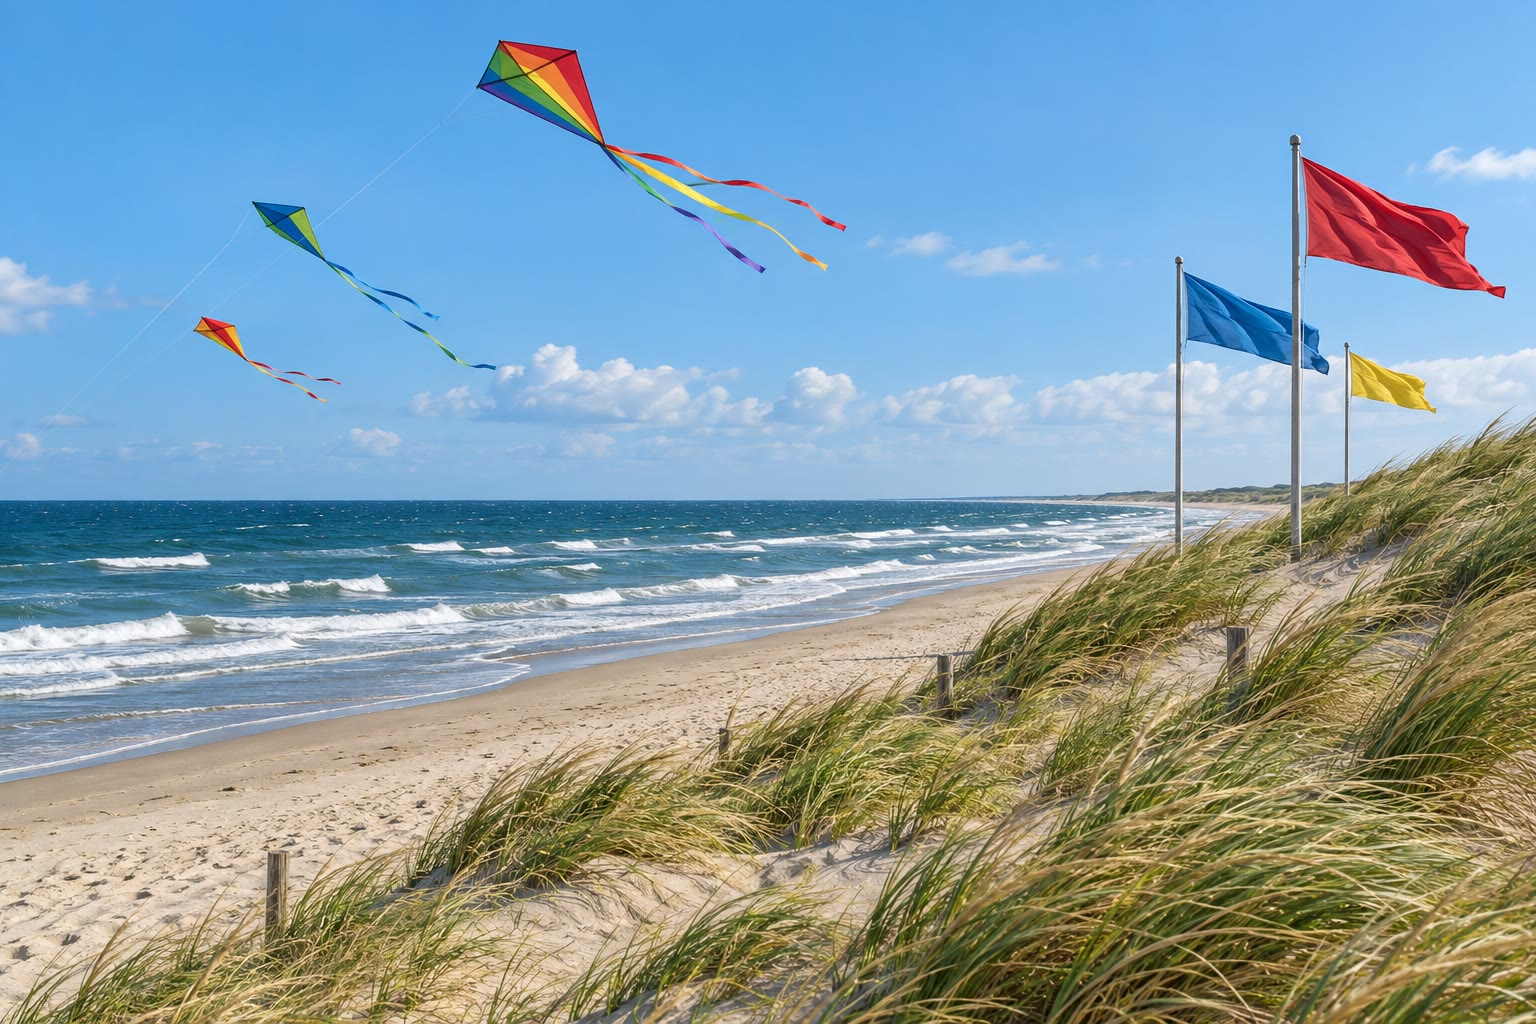
\includegraphics[width=0.55\linewidth]{images/book1/ai/g8-beach-kites.jpg}

{\small طائرات ورقية تحلّق في ريح ما بعد الظهر على شاطئ (رسم توضيحي مولَّد
بالذكاء الاصطناعي لمشهد عام).}
\label{fig:g8:winds-global-circulation:kites}
\end{omfigure}

\section{الرياح العامة}

يحدث الأمر نفسه على مقياس الأرض كلها. فقرب \omterm{def:g3:continents-and-oceans:equator}{خط الاستواء}، يصعد الهواء الشديد
السخونة؛ وينتشر نحو \omterm{def:g3:continents-and-oceans:poles}{القطبين} في الأعلى ثم يهبط من جديد قرب \omterm{def:g6:latitude-longitude:latitude}{دائرة العرض}
\ang{30}. وإذا أُخذ المتوسط على سنوات كثيرة، دار \omterm{def:g8:the-atmosphere:layers}{تروبوسفير} كل نصف كرة في ثلاث
\omterm{def:g8:winds-global-circulation:convection-cell}{خلايا حمل} كبرى: واحدة من \omterm{def:g3:continents-and-oceans:equator}{خط الاستواء} إلى نحو \ang{30}، وواحدة من نحو
\ang{30} إلى نحو \ang{60}، وواحدة من نحو \ang{60} إلى \omterm{def:g3:continents-and-oceans:poles}{القطب}. ويسميها خبراء
الأرصاد خلية هادلي وخلية فيريل والخلية القطبية. وحدودها تتحرك مع الفصول،
والخلية الوسطى متوسط تقريبي لعواصف كثيرة عابرة.
% ledger: mo:three-cells, mo:global-circ, nos:doldrums

لو لم تكن الأرض تدور، لهبت الرياح عند الأرض مباشرة من الضغط العالي إلى
الضغط المنخفض. لكن لأن الأرض تدور، ينحرف الهواء المتحرك: إلى اليمين في \omterm{def:g3:continents-and-oceans:equator}{نصف
الكرة الشمالي}، وإلى اليسار في \omterm{def:g3:continents-and-oceans:equator}{نصف الكرة الجنوبي}. ولذلك فإن الهواء العائد إلى
\omterm{def:g3:continents-and-oceans:equator}{خط الاستواء} لا يأتي من الشمال، بل من الشمال الشرقي في \omterm{def:g3:continents-and-oceans:equator}{نصف الكرة الشمالي}
ومن الجنوب الشرقي في \omterm{def:g3:continents-and-oceans:equator}{نصف الكرة الجنوبي}.
% ledger: mo:global-circ, nos:trade-winds

\begin{definition}[الرياح العامة]\label{def:g8:winds-global-circulation:global-winds}
الرياح السطحية التي تهب أكثر من غيرها في كل حزام من \omterm{def:g6:latitude-longitude:latitude}{دوائر العرض} هي:
\begin{itemize}
  \item \emph{الرياح التجارية}\index{رياح تجارية}، بين \omterm{def:g3:continents-and-oceans:equator}{خط الاستواء} ونحو
        \ang{30}، وتهب من الشمال الشرقي في \omterm{def:g3:continents-and-oceans:equator}{نصف الكرة الشمالي} ومن الجنوب
        الشرقي في \omterm{def:g3:continents-and-oceans:equator}{نصف الكرة الجنوبي}؛
  \item \emph{الرياح الغربية}\index{رياح غربية}، بين نحو \ang{30}
        و\ang{60}، وتهب من الغرب (من الجنوب الغربي في \omterm{def:g3:continents-and-oceans:equator}{نصف الكرة الشمالي}،
        ومن الشمال الغربي في الجنوبي)؛
  \item \emph{الرياح الشرقية القطبية}\index{رياح شرقية قطبية}، بين نحو
        \ang{60} \omterm{def:g3:continents-and-oceans:poles}{والقطبين}، وتهب من الشرق.
\end{itemize}
\end{definition}
% ledger: nos:trade-winds, mo:three-cells, mo:global-circ

\begin{omfigure}
\begin{tikzpicture}[font=\scriptsize, >={Stealth[length=1.8mm]}]
  \def\R{3}
  \fill[blue!8] (0,0) circle (\R);
  \draw (0,0) circle (\R);
  \draw[black!45] (-\R,0) -- (\R,0);
  \foreach \l in {-60,-30,30,60} {
    \pgfmathsetmacro{\y}{\R*sin(\l)}
    \pgfmathsetmacro{\x}{\R*cos(\l)}
    \draw[black!45, dashed] (-\x,\y) -- (\x,\y);}
  % surface winds: NE trades, SW westerlies, NE polar easterlies (north); mirrored south
  \foreach \x in {-1.8,-0.6,0.6,1.8} {
    \draw[->, omThm, line width=0.9pt] (\x+0.35,0.95) -- (\x-0.35,0.55);
    \draw[->, omThm, line width=0.9pt] (\x+0.35,-0.95) -- (\x-0.35,-0.55);}
  \foreach \x in {-1.2,0,1.2} {
    \draw[->, omDef, line width=0.9pt] (\x-0.35,1.7) -- (\x+0.35,2.02);
    \draw[->, omDef, line width=0.9pt] (\x-0.35,-1.7) -- (\x+0.35,-2.02);}
  \foreach \x in {-0.4,0.4} {
    \draw[->, omMeth, line width=0.9pt] (\x+0.25,2.85) -- (\x-0.25,2.65);
    \draw[->, omMeth, line width=0.9pt] (\x+0.25,-2.85) -- (\x-0.25,-2.65);}
  \node[fill=blue!8, inner sep=1pt] at (0,1.2) {الرياح التجارية الشمالية الشرقية};
  \node[fill=blue!8, inner sep=1pt] at (0,-1.2) {الرياح التجارية الجنوبية الشرقية};
  \node[fill=blue!8, inner sep=1pt] at (0,2.3) {الرياح الغربية};
  \node[fill=blue!8, inner sep=1pt] at (0,-2.3) {الرياح الغربية};
  \node[anchor=south] at (0,\R+0.05) {الرياح الشرقية القطبية};
  \node[anchor=north] at (0,-\R-0.05) {الرياح الشرقية القطبية};
  % pressure belts on the left
  \foreach \l/\t in {90/{ع: هواء هابط}, 60/{م: هواء صاعد}, 30/{ع: هواء هابط، جاف، صحارى}, 0/{م: هواء صاعد، سحب، مطر}, -30/{ع: هواء هابط، جاف، صحارى}, -60/{م: هواء صاعد}, -90/{ع: هواء هابط}} {
    \pgfmathsetmacro{\y}{\R*sin(\l)}
    \pgfmathsetmacro{\x}{\R*cos(\l)}
    \draw[black!40] (-\x-0.05,\y) -- (-3.35,\y);
    \node[anchor=east] at (-3.4,\y) {\t};}
  \foreach \l/\t in {60/{\foreignlanguage{arabic}{\mbox{\textdir TLT\ang{60}} ش}}, 30/{\foreignlanguage{arabic}{\mbox{\textdir TLT\ang{30}} ش}}, 0/{خط الاستواء}, -30/{\foreignlanguage{arabic}{\mbox{\textdir TLT\ang{30}} ج}}, -60/{\foreignlanguage{arabic}{\mbox{\textdir TLT\ang{60}} ج}}} {
    \pgfmathsetmacro{\y}{\R*sin(\l)}
    \pgfmathsetmacro{\x}{\R*cos(\l)}
    \node[anchor=west, black!60] at (\x+0.05,\y) {\t};}
  % side view of the cells (height to the right), same latitude scale
  \begin{scope}[xshift=5.2cm]
    \draw[->] (0,-\R) -- (0,\R+0.3);
    \draw (0,-\R) -- (1.8,-\R);
    \node[anchor=north, align=center] at (0.9,-\R-0.05) {الارتفاع في\\\foreignlanguage{arabic}{التروبوسفير $\rightarrow$}};
    \foreach \lo/\hi/\cw in {0/30/0, 30/60/1, 60/90/0, -30/0/1, -60/-30/0, -90/-60/1} {
      \pgfmathsetmacro{\ya}{\R*sin(\lo)}
      \pgfmathsetmacro{\yb}{\R*sin(\hi)}
      \pgfmathsetmacro{\yc}{(\ya+\yb)/2}
      \pgfmathsetmacro{\bb}{max(0.09,(\yb-\ya)/2-0.06)}
      \ifnum\cw=0
        \draw[black!70, line width=0.7pt, postaction={decorate}, decoration={markings,
          mark=at position 0.125 with {\arrow{Stealth[length=1.6mm]}}, mark=at position 0.375 with {\arrow{Stealth[length=1.6mm]}},
          mark=at position 0.625 with {\arrow{Stealth[length=1.6mm]}}, mark=at position 0.875 with {\arrow{Stealth[length=1.6mm]}}}]
          (0.9,\yc) ++(0.75,0) arc (0:360:0.75 and \bb);
      \else
        \draw[black!70, line width=0.7pt, postaction={decorate}, decoration={markings,
          mark=at position 0.125 with {\arrow{Stealth[length=1.6mm]}}, mark=at position 0.375 with {\arrow{Stealth[length=1.6mm]}},
          mark=at position 0.625 with {\arrow{Stealth[length=1.6mm]}}, mark=at position 0.875 with {\arrow{Stealth[length=1.6mm]}}}]
          (0.9,\yc) ++(0.75,0) arc (360:0:0.75 and \bb);
      \fi}
  \end{scope}
\end{tikzpicture}

{\small \omterm{def:g8:winds-global-circulation:circulation}{الدورة العامة}، مبسَّطة. على اليسار: أحزمة الضغط العالي (ع) والضغط
المنخفض (م) عند الأرض. وعلى الكرة: الرياح السطحية، التي يحرفها دوران الأرض.
وعلى اليمين: \omterm{def:g8:winds-global-circulation:convection-cell}{خلايا الحمل} الثلاث في كل نصف كرة كما تُرى من الجانب، عند \omterm{def:g6:latitude-longitude:latitude}{دوائر
العرض} نفسها (والخليتان القطبيتان مرسومتان رقيقتين جدًا لأن الحزام القطبي ضيق
على الكرة).}
% ledger: mo:three-cells, mo:global-circ, nos:trade-winds, nos:doldrums
\label{fig:g8:winds-global-circulation:cells}
\end{omfigure}

\begin{method}[إيجاد الريح العامة عند دائرة عرض]\label{met:g8:winds-global-circulation:wind}
\begin{enumerate}
  \item جد الحزام: من \omterm{def:g3:continents-and-oceans:equator}{خط الاستواء} إلى نحو \ang{30}، أو من \ang{30}
        إلى \ang{60}، أو من \ang{60} إلى \omterm{def:g3:continents-and-oceans:poles}{القطب}.
  \item جد الاتجاه الذي يتدفق فيه الهواء عند الأرض في ذلك الحزام: نحو
        \omterm{def:g3:continents-and-oceans:equator}{خط الاستواء} في الحزام الأول والأخير، ونحو \omterm{def:g3:continents-and-oceans:poles}{القطب} في الحزام
        الأوسط.
  \item احرف هذا التدفق: إلى اليمين في \omterm{def:g3:continents-and-oceans:equator}{نصف الكرة الشمالي}، وإلى
        اليسار في \omterm{def:g3:continents-and-oceans:equator}{نصف الكرة الجنوبي}.
  \item قل من أين تأتي الريح: فالرياح تُسمّى بالاتجاه الذي تهب
        \emph{منه}.
\end{enumerate}
\end{method}

\begin{example}[الريح عند \ang{40} جنوبًا]\label{ex:g8:winds-global-circulation:40s}
عند \ang{40} جنوبًا نكون في الحزام الأوسط، بين \ang{30} و\ang{60}.
وهناك يتدفق الهواء عند الأرض نحو \omterm{def:g3:continents-and-oceans:poles}{القطب}، أي نحو الجنوب. وفي \omterm{def:g3:continents-and-oceans:equator}{نصف الكرة الجنوبي}
ينحرف إلى اليسار: وللهواء المتجه جنوبًا، اليسار هو الشرق، فينتهي الهواء
متحركًا نحو الجنوب الشرقي. فهو إذن يأتي من الشمال الغربي: إنه من \omterm{def:g8:winds-global-circulation:global-winds}{الرياح
الغربية}، ويهب من الشمال الغربي.
\end{example}
% ledger: mo:three-cells, mo:global-circ

قرب \omterm{def:g3:continents-and-oceans:equator}{خط الاستواء}، حيث تلتقي \omterm{def:g8:winds-global-circulation:global-winds}{الرياح التجارية} لنصفي الكرة، تخمد الرياح: وقد
سمى البحارة هذا الحزام الهادئ \emph{الركود الاستوائي}. فالهواء الدافئ الرطب
يصعد هناك، ويبرد ويعطي زخات مستمرة وعواصف رعدية. وقرب \ang{30}، تحت
الهواء الهابط، تكون الرياح خفيفة \omterm{def:g4:clouds-rain-snow:precipitation}{والمطر} نادرًا.
% ledger: nos:doldrums

\begin{definition}[الدورة العامة للغلاف الجوي]\label{def:g8:winds-global-circulation:circulation}
\emph{الدورة العامة}\index{دورة عامة} للغلاف الجوي هي حركة الهواء الواسعة
النطاق حول الكوكب، كما تظهر حين يُؤخذ متوسط الرياح على سنوات كثيرة. وهي
تنقل الحرارة من \omterm{def:g3:continents-and-oceans:equator}{خط الاستواء} نحو \omterm{def:g3:continents-and-oceans:poles}{القطبين}، وبخار الماء من حزام عرض إلى
آخر.
\end{definition}
% ledger: mo:global-circ

\section{الدورة العامة والنطاقات المناخية}

تفسر \omterm{def:g8:winds-global-circulation:circulation}{الدورة العامة} جزءًا كبيرًا من \omterm{def:g2:drawing-to-map:map}{خريطة} المناخات. فحيث يصعد الهواء، قرب
\omterm{def:g3:continents-and-oceans:equator}{خط الاستواء}، يبرد ويتحول بخار الماء الذي فيه إلى \omterm{def:g4:clouds-rain-snow:cloud}{سحب}: فيكثر \omterm{def:g4:clouds-rain-snow:precipitation}{المطر}، وتنمو
\omterm{def:g5:weather-and-climate:rainforest}{الغابات المطيرة}. وحيث يهبط الهواء، قرب \ang{30} شمالًا وجنوبًا، يسخن وهو
ينزل، وتتبدد سحبه، ويندر \omterm{def:g4:clouds-rain-snow:precipitation}{المطر}: ففي هذين الحزامين تقع \omterm{def:g5:weather-and-climate:desert}{الصحارى} الحارة
الكبرى، مثل \omterm{def:g5:weather-and-climate:desert}{الصحراء} الكبرى. وفي العروض الوسطى، تجلب \omterm{def:g8:winds-global-circulation:global-winds}{الرياح الغربية} \omterm{def:g5:natural-hazards:storm}{عاصفة}
بعد \omterm{def:g5:natural-hazards:storm}{عاصفة}، مع \omterm{def:g4:clouds-rain-snow:precipitation}{مطر} في كل الفصول.
% ledger: nos:doldrums, mo:three-cells, mo:global-circ

\begin{omfigure}
\begin{minipage}[c]{0.42\linewidth}\centering
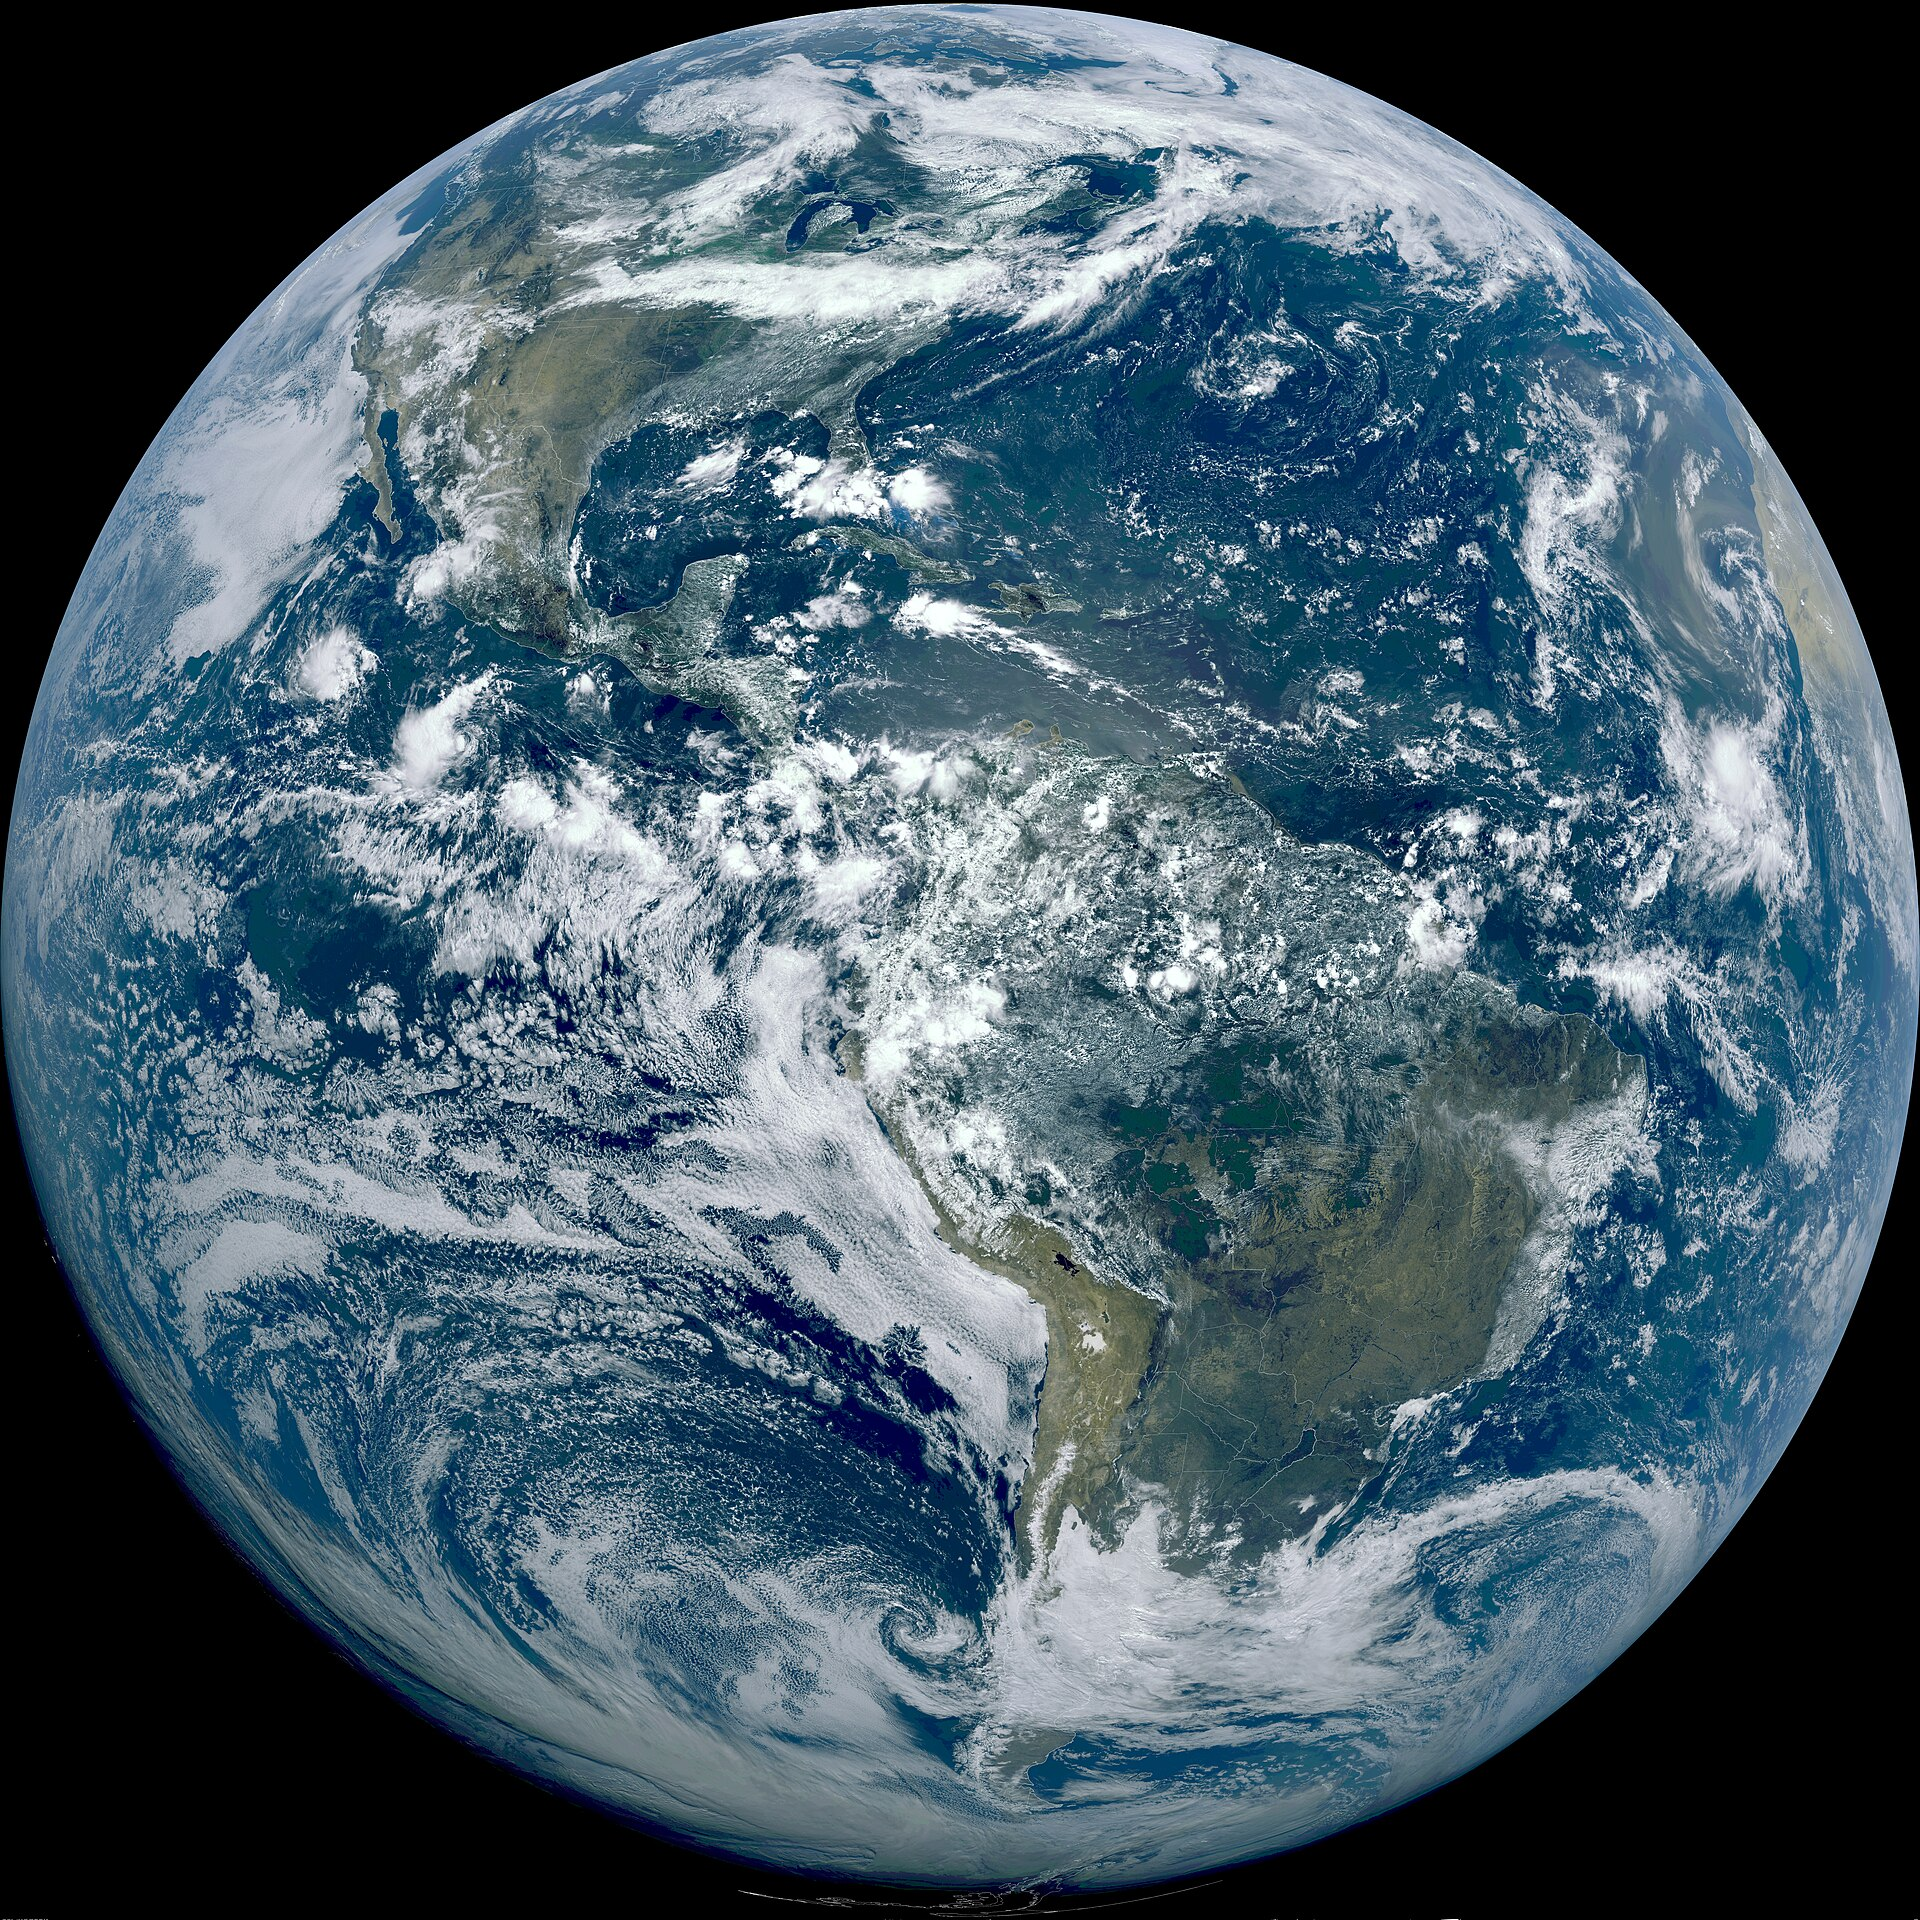
\includegraphics[width=\linewidth]{images/book1/g8-goes-full-disk.jpg}
\end{minipage}\hfill
\begin{minipage}[c]{0.54\linewidth}\raggedright
{\small الأمريكيتان كما يراهما القمر الصناعي لرصد \omterm{def:g1:watching-the-weather:weather}{الطقس} غويس-16، عاليًا فوق
\omterm{def:g3:continents-and-oceans:equator}{خط الاستواء}، في 26~يوليو 2022. فقد تكونت \omterm{def:g4:clouds-rain-snow:cloud}{سحب} كثيرة فوق المنطقة المدارية
وغابة الأمازون المطيرة، حيث يصعد الهواء الدافئ الرطب؛ وبعيدًا في الجنوب،
في شتاء \omterm{def:g3:continents-and-oceans:equator}{نصف الكرة الجنوبي}، تدور عواصف \omterm{def:g8:winds-global-circulation:global-winds}{الرياح الغربية} فوق \omterm{def:g2:water-on-earth:ocean}{المحيط}. الإدارة
الوطنية للمحيطات والغلاف الجوي (ملك عام، عبر ويكيميديا كومنز).}
\end{minipage}
% ledger: commons:goes16, nos:doldrums
\label{fig:g8:winds-global-circulation:goes}
\end{omfigure}

\begin{example}[أربع مدن، أربعة أحزمة]\label{ex:g8:winds-global-circulation:four-towns}
المدن الأربع التي في \omterm{def:g5:weather-and-climate:climate-chart}{المخططات المناخية} في \cref{ch:g5:weather-and-climate}
تقع كلها في \omterm{def:g3:continents-and-oceans:equator}{نصف الكرة الشمالي}، على \omterm{def:g6:latitude-longitude:latitude}{دوائر عرض} مختلفة جدًا. ومطرها وثلجها
السنويان يتبعان أحزمة \omterm{def:g8:winds-global-circulation:circulation}{الدورة العامة} (المخطط أدناه). فهيلو، عند \ang{20}
شمالًا، تقع على جزيرة في حزام \omterm{def:g8:winds-global-circulation:global-winds}{الرياح التجارية}، في وسط \omterm{def:g2:water-on-earth:ocean}{المحيط}، حيث تحمل
\omterm{def:g8:winds-global-circulation:global-winds}{الرياح التجارية} بخار الماء: فيسقط فيها نحو \qty{3000}{mm} في السنة. وفينيكس،
عند \ang{33} شمالًا، تقع قرب \ang{30}، تحت الهواء الهابط: أقل من
\qty{200}{mm}. وسياتل، عند \ang{47} شمالًا، في \omterm{def:g8:winds-global-circulation:global-winds}{الرياح الغربية}، التي تجلب
عواصفها نحو \qty{1000}{mm} في السنة، معظمها من الخريف إلى الربيع. وأوتكياغفيك،
عند \ang{71} شمالًا، تقع تحت الهواء البارد الذي يهبط قرب \omterm{def:g3:continents-and-oceans:poles}{القطب}: أقل من
\qty{150}{mm}، فهي \omterm{def:g5:weather-and-climate:desert}{صحراء} باردة.
% ledger: data:b1-noaa-normals (totals from figdata/grade-5/climate_charts.py, re-read in figdata/grade-8/rain_by_belt.py), mo:three-cells, nos:doldrums
\end{example}

\begin{omfigure}
\begin{tikzpicture}
\begin{axis}[xbar, width=0.82\linewidth, height=6.4cm, bar width=9pt,
  xmin=0, xmax=3600, ymin=0, ymax=90, ytick={0,30,60,90},
  yticklabels={$0^\circ$, \foreignlanguage{arabic}{$30^\circ$ ش}, \foreignlanguage{arabic}{$60^\circ$ ش}, \foreignlanguage{arabic}{$90^\circ$ ش}},
  xlabel={\foreignlanguage{arabic}{المطر والثلج في السنة \babelsublr{(mm)}}}, ylabel={دائرة العرض},
  axis x line=bottom, axis y line=left, axis line style={-},
  tick label style={font=\scriptsize}, label style={font=\small},
  xtick={0,1000,2000,3000}, scaled x ticks=false, clip=false,
  ]
  \draw[black!35, dashed] (axis cs:0,30) -- (axis cs:3600,30);
  \draw[black!35, dashed] (axis cs:0,60) -- (axis cs:3600,60);
  \node[font=\scriptsize, black!60, anchor=south east] at (axis cs:3600,1) {هواء صاعد: مطر};
  \node[font=\scriptsize, black!60, anchor=south east] at (axis cs:3600,30) {هواء هابط: جفاف};
  \node[font=\scriptsize, black!60, anchor=south east] at (axis cs:3600,60) {هواء صاعد: مطر};
  \node[font=\scriptsize, black!60, anchor=north east] at (axis cs:3600,90) {هواء هابط: جفاف};
  \addplot[fill=blue!35, draw=blue!60!black] table[x=total_mm, y=lat] {figdata/out/grade-8-rain_by_belt-stations.dat};
  \node[font=\scriptsize, anchor=west] at (axis cs:3058,19.72) {هيلو};
  \node[font=\scriptsize, anchor=west] at (axis cs:183,33.43) {فينيكس};
  \node[font=\scriptsize, anchor=west] at (axis cs:999,47.44) {سياتل};
  \node[font=\scriptsize, anchor=west] at (axis cs:137,71.28) {أوتكياغفيك};
\end{axis}
\end{tikzpicture}

{\small \omterm{def:g4:clouds-rain-snow:precipitation}{المطر} \omterm{def:g4:clouds-rain-snow:precipitation}{والثلج} السنويان (متوسطات 1991--2020) للمدن الأربع التي في
\omterm{def:g5:weather-and-climate:climate-chart}{المخططات المناخية}، موضوعةً عند دوائر عرضها. فالمدن الرطبة تقع حيث يصعد
الهواء، قرب \omterm{def:g3:continents-and-oceans:equator}{خط الاستواء} وقرب \ang{60}؛ والجافة حيث يهبط، قرب \ang{30}
وقرب \omterm{def:g3:continents-and-oceans:poles}{القطب}. المعدلات المناخية للإدارة الوطنية للمحيطات والغلاف الجوي.}
% ledger: data:b1-noaa-normals, mo:three-cells (figdata/grade-8/rain_by_belt.py)
\end{omfigure}

أربع مدن ليست إلا أربع نقاط: \omterm{def:g1:landscapes-around-us:landform}{فالجبال} \omterm{def:g1:landscapes-around-us:water}{والسواحل} والبحار الباردة أو الدافئة
تغير هي أيضًا مقدار \omterm{def:g4:clouds-rain-snow:precipitation}{المطر} الذي يتلقاه مكان ما. والأحزمة تعطي النمط العام
\omterm{def:g2:drawing-to-map:map}{لخريطة} المناخات، لا \omterm{def:g4:clouds-rain-snow:precipitation}{مطر} كل مدينة.

\section{تمارين}

\begin{exercise}[$\star$]\label{exo:g8:winds-global-circulation:1}
سمِّ الريح العامة التي تهب أكثر من غيرها: (أ) عند \ang{15} شمالًا؛
(ب) عند \ang{45} جنوبًا؛ (ج) عند \ang{75} شمالًا؛ (د) عند \ang{20} جنوبًا.
وأعطِ اتجاهها في كل مرة.
\end{exercise}

\begin{exercise}[$\star$]\label{exo:g8:winds-global-circulation:2}
أكمل كل جملة. (أ) الهواء الدافئ \dots\ والهواء البارد \dots. (ب) تحت
الهواء الصاعد، يكون الضغط عند الأرض \dots. (ج) عند الأرض، تهب الريح من
الضغط \dots\ نحو الضغط \dots. (د) في \omterm{def:g3:continents-and-oceans:equator}{نصف الكرة الشمالي}، يحرف دوران الأرض
الهواء المتحرك إلى \dots.
\end{exercise}

\begin{exercise}[$\star$]\label{exo:g8:winds-global-circulation:3}
صواب أم خطأ؟ صحّح الجمل الخاطئة. (أ) يهب \omterm{def:g8:winds-global-circulation:breezes}{نسيم البحر} من اليابسة إلى
\omterm{def:g2:water-on-earth:ocean}{البحر}. (ب) تسخن اليابسة أسرع من \omterm{def:g2:water-on-earth:ocean}{البحر} في النهار. (ج) تهب \omterm{def:g8:winds-global-circulation:global-winds}{الرياح التجارية}
من الغرب. (د) كثير من \omterm{def:g5:weather-and-climate:desert}{الصحارى} الكبرى تقع قرب \omterm{def:g6:latitude-longitude:latitude}{دائرة العرض}
\ang{30}.
\end{exercise}

\begin{exercise}[$\star$]\label{exo:g8:winds-global-circulation:4}
ارسم ساحلًا \omterm{def:g2:water-on-earth:ocean}{والبحر} على اليسار واليابسة على اليمين. أضف الشمس، ثم ارسم
بالأسهم حلقة الهواء \omterm{def:g8:winds-global-circulation:breezes}{لنسيم البحر}. وضع الحرفين ع وم حيث يكون الضغط عند
الأرض عاليًا ومنخفضًا.
\end{exercise}

\begin{exercise}[$\star\star$]\label{exo:g8:winds-global-circulation:5}
استعمل جدول الحزم في هذا الفصل. (أ) عند \ang{45}، كم مرة تزيد الأرض التي
تغطيها الحزمة على ما تغطيه عند \omterm{def:g3:continents-and-oceans:equator}{خط الاستواء}؟ (ب) ما النسبة المئوية من طاقة
\omterm{def:g3:continents-and-oceans:equator}{خط الاستواء} التي يتلقاها كل متر مربع عند \ang{60}؟ (ج) وعند
\ang{75}؟ (د) اشرح في جملة واحدة لماذا القطبان باردان.
\end{exercise}

\begin{exercise}[$\star\star$]\label{exo:g8:winds-global-circulation:6}
يبحر قارب جنوبًا تمامًا عبر \omterm{def:g3:continents-and-oceans:equator}{نصف الكرة الشمالي} ثم \omterm{def:g3:continents-and-oceans:equator}{نصف الكرة الجنوبي}. (أ) ما
الرياح التي يصادفها، بالترتيب، من \ang{70} شمالًا إلى \ang{70} جنوبًا؟
(ب) أين يُرجَّح أن يجد هواء هادئًا وزخات متكررة؟ (ج) أين تكون الرياح
خفيفة \omterm{def:g4:clouds-rain-snow:precipitation}{والمطر} نادرًا؟
\end{exercise}

\begin{exercise}[$\star\star$]\label{exo:g8:winds-global-circulation:7}
على شاطئ، تبلغ درجة الحرارة \qty{31}{\degreeCelsius} فوق \omterm{def:g3:stones-pebbles-sand:sand}{الرمل} في الساعة 3
بعد الظهر و\qty{22}{\degreeCelsius} فوق \omterm{def:g2:water-on-earth:ocean}{البحر}. وفي الساعة 3 فجرًا تبلغ
\qty{17}{\degreeCelsius} فوق اليابسة و\qty{21}{\degreeCelsius} فوق
\omterm{def:g2:water-on-earth:ocean}{البحر}. (أ) أيهما أدفأ في الساعة 3 بعد الظهر؟ وفي أي اتجاه تهب الريح؟
(ب) وفي الساعة 3 فجرًا؟ (ج) بكم درجة تتغير درجة حرارة اليابسة بين الوقتين؟
وبكم تتغير درجة حرارة \omterm{def:g2:water-on-earth:ocean}{البحر}؟ (د) اشرح الفرق.
\end{exercise}

\begin{exercise}[$\star\star$]\label{exo:g8:winds-global-circulation:8}
يتدفق الهواء من حزام الضغط العالي قرب \ang{30} شمالًا نحو \omterm{def:g3:continents-and-oceans:equator}{خط الاستواء}.
(أ) لو لم تكن الأرض تدور، فمن أي اتجاه كان سيهب؟ (ب) إلى أي جهة يحرفه
الدوران في \omterm{def:g3:continents-and-oceans:equator}{نصف الكرة} هذا؟ (ج) من أي اتجاه يهب إذن؟ (د) أجب عن الأسئلة
الثلاثة نفسها للهواء المتدفق نحو \omterm{def:g3:continents-and-oceans:equator}{خط الاستواء} من \ang{30} جنوبًا.
\end{exercise}

\begin{exercise}[$\star\star$]\label{exo:g8:winds-global-circulation:9}
اشرح، خطوة خطوة، لماذا يكثر \omterm{def:g4:clouds-rain-snow:precipitation}{المطر} قرب \omterm{def:g3:continents-and-oceans:equator}{خط الاستواء}:
استعمل الكلمات \emph{يسخن}، \emph{يصعد}، \emph{يبرد}، \emph{\omterm{def:g4:clouds-rain-snow:cloud}{سحب}}.
ثم اشرح لماذا توجد \omterm{def:g5:weather-and-climate:desert}{صحراء} قرب \ang{25} شمالًا في شمال إفريقيا: استعمل
الكلمات \emph{يهبط}، \emph{ضغط عالٍ}، \emph{جاف}.
\end{exercise}

\begin{exercise}[$\star\star$]\label{exo:g8:winds-global-circulation:10}
تغادر سفينة شراعية ميناء عند \ang{40} شمالًا على \omterm{def:g1:landscapes-around-us:water}{الساحل} الغربي لأوروبا
متجهة إلى \omterm{def:g2:water-on-earth:ocean}{البحر} الكاريبي، عند \ang{15} شمالًا. (أ) أي ريح ستصادف عند
\ang{40} شمالًا؟ وهل تساعد السفينة على الإبحار غربًا؟ (ب) لماذا ينبغي
للسفينة أن تبحر جنوبًا أولًا؟ (ج) أي ريح تحملها غربًا، وبين أي
دائرتي عرض؟ (د) في رحلة العودة إلى أوروبا، أي ريح ينبغي للسفينة أن
تبحث عنها، وعند أي دائرة عرض؟
\end{exercise}

\begin{exercise}[$\star\star\star$]\label{exo:g8:winds-global-circulation:11}
عند \omterm{def:g6:latitude-longitude:latitude}{دائرة العرض} $L$، تغطي حزمة من ضوء الشمس عند الظهر في يوم الاعتدال $1 \div
\cos L$ ضعفًا من الأرض التي تغطيها عند \omterm{def:g3:continents-and-oceans:equator}{خط الاستواء} (وعلى الآلة الحاسبة،
$\cos 60^\circ = 0.5$). (أ) تحقق من القيمة عند \ang{60}. (ب) باستعمال
$\cos 30^\circ \approx 0.866$، تحقق من القيمة عند \ang{30}، مقرَّبة إلى
رقمين عشريين. (ج) افترض أن لوحًا شمسيًا مستويًا يتلقى
\qty{1000}{W} على كل متر مربع عند الظهر عند \omterm{def:g3:continents-and-oceans:equator}{خط الاستواء} في ذلك اليوم.
فكم يتلقى اللوح نفسه تقريبًا عند \ang{30}؟ وعند \ang{60}؟
\end{exercise}

\begin{exercise}[$\star\star\star$]\label{exo:g8:winds-global-circulation:12}
في كل نصف كرة، \omterm{def:g8:winds-global-circulation:circulation}{للدورة العامة} ثلاث خلايا. (أ) ارسم منظرًا جانبيًا \omterm{def:g3:continents-and-oceans:equator}{لنصف
الكرة الشمالي}، \omterm{def:g3:continents-and-oceans:equator}{وخط الاستواء} في الأسفل \omterm{def:g3:continents-and-oceans:poles}{والقطب} في الأعلى، والخلايا الثلاث
حلقات؛ وبيّن أين يصعد الهواء وأين يهبط. (ب) حدد أحزمة الضغط العالي
والمنخفض عند الأرض. (ج) أضف الرياح السطحية لكل خلية، منحرفة إلى اليمين.
(د) استعمل رسمك لتشرح لماذا تهب \omterm{def:g8:winds-global-circulation:global-winds}{الرياح الغربية} نحو
الشمال الشرقي.
\end{exercise}

\section{مسألة: الإبحار مع الرياح التجارية}

\begin{problem}[{مسألة نهاية الأسبوع --- سفينة شراعية تعبر الأطلسي من الرأس
الأخضر إلى بربادوس مع الريح التجارية الشمالية الشرقية؛ يُقاس الطريق على
الخريطة، وتُقرأ الريح، ويُحسب طول العبور}]
\label{pb:g8:winds-global-circulation:1}
% ledger: data:b1-ne-places, earth:Rmean, nos:trade-winds (figdata/grade-8/trade_route.py; the speed is exercise data)
تغادر سفينة شراعية برايا، في جزر الرأس الأخضر، متجهة إلى بريدجتاون، في
بربادوس. وتُظهر \omterm{def:g2:drawing-to-map:map}{الخريطة} الطريق والريح التجارية.

\begin{center}
\begin{tikzpicture}
\begin{axis}[ommap, width=12cm, xmin=-75, xmax=-5, ymin=0, ymax=35, axis equal image,
  xtick={-70,-60,-50,-40,-30,-20,-10}, ytick={0,10,20,30},
  tick label style={font=\scriptsize},
  xlabel={\foreignlanguage{arabic}{خط الطول، والسالب يعني الغرب}}, ylabel={\foreignlanguage{arabic}{دائرة العرض شمالًا}},
  label style={font=\small}, clip mode=individual]
  \addplot[fill=omLithAlluv, draw=black!60, line width=0.3pt] table {figdata/out/grade-8-trade_route-land.dat};
  \addplot[quiver={u=\thisrow{dlon}, v=\thisrow{dlat}}, -{Stealth[length=1.6mm]}, omThm!80, line width=0.7pt]
    table[x=lon, y=lat] {figdata/out/grade-8-trade_route-trades.dat};
  \addplot[omDef, line width=1.3pt, dashed] table {figdata/out/grade-8-trade_route-route.dat};
  \addplot[only marks, mark=*, mark size=2pt, black] table[x=lon, y=lat] {figdata/out/grade-8-trade_route-ports.dat};
  \node[anchor=north, font=\scriptsize\bfseries, fill=white, inner sep=1pt] at (axis cs:-59.6,12.2) {بريدجتاون};
  \node[anchor=south, font=\scriptsize\bfseries, fill=white, inner sep=1pt] at (axis cs:-23.5,15.8) {برايا};
\end{axis}
\end{tikzpicture}
\end{center}

\noindent\textbf{الجزء الأول --- الطريق.}\par\nopagebreak
\begin{enumerate}[beginpenalty=10000]
  \item تقع برايا عند \ang{14.9} شمالًا، \ang{23.5} غربًا؛ وبريدجتاون عند
        \ang{13.1} شمالًا، \ang{59.6} غربًا. كم درجة من \omterm{def:g6:latitude-longitude:longitude}{خطوط الطول}
        تفصل بينهما؟
  \item يقع الميناءان كلاهما قرب \ang{14} شمالًا. وعلى طول \omterm{def:g6:latitude-longitude:latitude}{دائرة العرض} هذه،
        تقيس الدرجة الواحدة من \omterm{def:g6:latitude-longitude:longitude}{خط الطول} نحو \qty{108}{km}. فكم كيلومترًا
        يبلغ العبور تقريبًا؟ قرّب إلى أقرب مئة.
  \item إذا قيس الطريق الأقصر قياسًا دقيقًا على الأرض الكروية، بلغ
        \qty{3896}{km}. فهل إجابة السؤال 2 تقدير جيد؟
  \item هل يقع الميناءان في حزام \omterm{def:g8:winds-global-circulation:global-winds}{الرياح التجارية}؟ اشرح.
\end{enumerate}

\noindent\textbf{الجزء الثاني --- الريح.}\par\nopagebreak
\begin{enumerate}[resume, beginpenalty=10000]
  \item من أي اتجاه تهب الريح التجارية هنا؟
  \item تبحر السفينة نحو الغرب. هل تدفعها الريح إلى الأمام، أم إلى الخلف،
        أم جانبيًا؟ اشرح بالاستعانة \omterm{def:g2:drawing-to-map:map}{بالخريطة}.
  \item لماذا تهب الريح التجارية في الاتجاه نفسه تقريبًا كل يوم
        من أيام العبور؟
  \item في طريق العودة إلى أوروبا، لماذا لا ينبغي للربان أن يحاول
        الإبحار شرقًا على طول \ang{14} شمالًا؟
\end{enumerate}

\noindent\textbf{الجزء الثالث --- العبور.}\par\nopagebreak
\begin{enumerate}[resume, beginpenalty=10000]
  \item افترض أن متوسط سرعة السفينة \qty{7}{km} في الساعة. فكم
        كيلومترًا تقطع في يوم من 24 ساعة؟
  \item لو خمدت الريح 3 أيام أثناء الطريق، فكم
        كيلومترًا من التقدم ستخسر السفينة؟
  \item مع ريح تجارية ثابتة، كم يومًا تحتاج السفينة لقطع
        \qty{3896}{km}؟ قرّب إلى رقم عشري واحد.
  \item كم يدوم العبور، مقرَّبًا إلى أقرب يوم كامل؟ وهل هو أكثر من
        شهر أم أقل؟
\end{enumerate}
\end{problem}
